%

\documentclass[runningheads]{llncs}
\usepackage[english,brazil]{babel}
%
\usepackage{graphicx}
% Used for displaying a sample figure. If possible, figure files should
% be included in EPS format.
%
% If you use the hyperref package, please uncomment the following line
% to display URLs in blue roman font according to Springer's eBook style:
% \renewcommand\UrlFont{\color{blue}\rmfamily}

\begin{document}
%
\title{Sistema Minix 3}
%
%\titlerunning{Abbreviated paper title}
% If the paper title is too long for the running head, you can set
% an abbreviated paper title here
%
\author{Ubiratan de Oliveira Júnior - ubiratan@alu.ufc.br}
%
\authorrunning{}
% First names are abbreviated in the running head.
% If there are more than two authors, 'et al.' is used.
%
\institute{Universidade Federal do Ceará}
%
\maketitle              % typeset the header of the contribution
%
\begin{abstract}
Artigo preparado para a disciplina de Sistemas Operacionais com a finalidade de resumir e sumarizar informações importantes sobre o sistema Minix 3, tais como o funcionamento de seu kernel, vantagens e desvantagens e comparativo com outros sistemas Unix like.

\end{abstract}
\keywords{\and Kernel \and Linux \and Microkernel \and Minix 3 \and Unix \and POSIX}

\section{Introdução}    
O Minix é um SO gratuito desenvolvido por Andrew Tanenbaum para compensar a proibição da AT\&T  contra o estudo de SO's baseados no código UNIX e prover uma ferramenta de ensino para seus alunos. Originalmente foi projetado para ser compatível com a versão 7 do UNIX e em seguida passou a ser desenvolvido baseado no padrão POSIX. 
O Minix foi escrito a partir do zero e mesmo sendo compatível com UNIX, não contém código AT\&T possibilitando sua distribuição livremente.

\section{Trabalhos Relacionados}
\subsection{MINIX 3: status report e pesquisas atuais}Inicialmente pensado como um sistema exclusivamente para experimentos e estudos acadêmicos (MINIX 1), o MINIX 3 é um S.O maduro com uma arquitetura que o torna altamente disponível e tolerante a falhas e mantém bem definida a API POSIX. 

\paragraph*{}A visão do MINIX 3 é baseada nos seguintes princípios:
\begin{itemize}
\item \textbf{Separação de preocupações}: Divida o sistema operacional em componentes bem isolados uns dos outros.
\item \textbf{Menos autoridade}: Conceda a cada componente apenas os poderes necessários para realizar seu trabalho e não mais que isso.
\item \textbf{Tolerância a falhas}: Admita a existência de bugs e planeje recuperá-los enquanto continua a execução.
\item \textbf{Atualização dinâmica}: Planeje ficar ativo o tempo todo, mesmo diante de grandes atualizações de software.
\item \textbf{Conformidade com os padrões}: Esteja em conformidade com o POSIX externamente, mas não tenha medo de mudanças internas.
\end{itemize}

\subsection{Reorganizando o UNIX para Confiabilidade}O MINIX 3 apresenta seus principais componentes de kernel executados em modo usuário, sendo eles: Sistema de arquivos (FS). Gerenciamento de processos (PM). Gerenciamento de memória (MM). Armazenamento de dados (DS), que é um pequeno servidor de banco de dados com funcionalidade de publish-subscribe. Finalmente, o servidor de reencarnação (RS) que rastreia todos os componentes e drivers e pode reparar de forma transparente o sistema quando certas falhas ocorrem.

\begin{figure}[h]
    \centering
    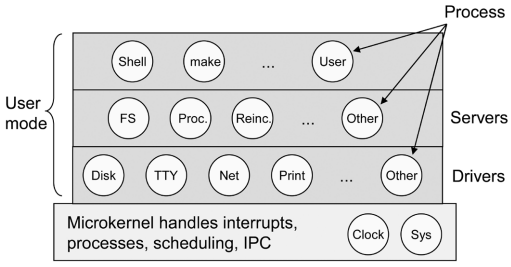
\includegraphics[width=9cm, height=5cm]{MINIX ARCH.png}
    \caption{Ilustração da arquitetura do MINIX 3.}
\end{figure}

\paragraph*{}Uma das vantagens da reorganização é a criação de barreiras de proteção entre os módulos, devido ao uso de drivers e funcionalidades do sistemas fora do Kernel através de processos em modo de usuário e sem privilégios.
O uso desses compartimentos aumenta a confiabilidade do sistema pois é fornecido um isolamento entre as falhas dos componentes, viabilizando um modelo de reinicialização mais eficiente, onde é feita a reinicialização de componentes e não do sistema completo.

\paragraph*{Isolamento de Falhas}O kernel junto com a unidade de gerenciameto de memória (MMU) garantem que os processos estejam isolados através de uma estratégia de emcapsulamento utilizando endereços privados de espaço. O acesso a áreas
restritas de memória só é possível quando são utilizados descritores de capaicidade atribuidos a um processo, que utiliza as funcionalidades de cópia do Kernel para realizar ações mais sensíveis.

\paragraph*{Tolerância a Falhas}Como os sitemas não estão a salvos de bugs e comportamentos inesperados de quem os opera, o servidor RS executa um script de política quando detecta uma falha e
pode substituir automaticamente um processo de sistema com falha por uma nova cópia Ao lado do RS, o DS é parte integrante do modelo de tolerância a falhas, seu mecanismo de publish-subscribe o torna muito adequado para informar outros processos de mudanças no sistema operacional. Por exemplo, FS assina o identificador para os drivers de disco. Quando um driver trava e o RS registra um novo, o DS notifica FS sobre o evento; O FS então pode tomar outras medidas para se recuperar da falha.

\section{ O Poder do Microkernel }
\subsection{Organização}

\subsection{Segurança}

\subsection{Desempenho}


\begin{thebibliography}{8}
\bibitem{ref_article1}
Jorrit N. Herder, Herbert Bos, Ben Gras, Philip Homburg, and Andrew S. Tanenbaum.: Reorganizing UNIX for Reliability. In:  Proc. 11th Asia-Pacific Computer Systems Architecture Conf. (ACSAC '06), pp. 81–94, Shanghai, China, Sep. 2006.

\bibitem{ref_lncs1}
Andrew Tanenbaum, Raja Appuswamy, Herbert Bos, Lorenzo Cavallaro, Cristiano Giuffrida, Tomás Hrubý, Jorrit Herder, Erik Van Der Kouwe, and David Van Moolenbroek.: MINIX 3: status report and current research; Login: June 2010

\end{thebibliography}
\end{document}
